\chapter{Desarrollo}

% Conceptos Básicos
\section{Conceptos Básicos}
    La \textbf{complejidad temporal}, dentro del análisis de algoritmos, es el número de operaciones que ejecuta un algoritmo en cierto tiempo. Su denotación es T(n) y puede ser analizada mediante dos tipos de análisis:
    
    \begin{itemize}
        \item Análisis de priori: entrega una función que muestra el tiempo de cálculo de un algoritmo.
        \item Análisis a posteriori: es la prueba en tiempo real del algoritmo, midiendo su costo mediante valores de entrada. 
    \end{itemize}
    
    El análisis de complejidad temporal define que un algoritmo alcanza su máximo potencial cuando los valores de entrada son mayores al tiempo estimado de ejecución, siendo que es factible poder completar sus ejecuciones en menor tiempo posible. 
    
    \textbf{Algoritmo Strassen} Es un algoritmo para la multiplicación de matrices. Es más rápido que el algoritmo estándar de multiplicación de matrices y es útil en la práctica para matrices grandes, pero sería más lento que los algoritmos más rápidos conocidos para matrices extremadamente grandes. Calcula el producto de dos matrices cuadradas de tamaño n \cite{Strassen}.

    \textbf{Teorema Maestro} Es una técnica para las recurrencias de divide y vencerás proporciona un análisis asintótico para las relaciones de recurrencia de tipos que ocurren en el análisis de muchos algoritmos de divide y vencerás \cite{TM}.
    
    
    
    
\newpage
\section{Algoritmo Rotación Imagen}
    \subsection{Algoritmo Rotación Imagen}
   
    \subsubsection{Pseudocódigo Algoritmo Rotación Imagen}
    El algoritmo consta de rota una imagen 90 grados hacia la izquierda partiendo de dividir la imagen en sectores de pixeles, obteniendo sus matrices RGB. Aplicando Divide y Vencerás se parte el problema en pequeños subproblemas para rotar la imagen. El proceso del algoritmo es obtener el \textit{width y height} (el ancho y largo respectivamente) del sector, hace un análisis, si ambas medidas son iguales a 1 hace la rotación de pixeles sin entrar en el proceso recursivo. En caso contrario, de no existir cuadrantes en la imagen, divide en  4 cuadrantes que serán rotados usando recursividad, la función recibe como parametro el sector y la rotación, esto en cada paso de la recursividad se realiza hasta que el sector sea lo suficientemente pequeño para rotar cada pixel de cada cuadrante. Al final intercambia cuadrantes para hacer el cambio de rotación, finalizando con la unión de los cuadrantes en la imagen final. En la figura \ref{fig:ejemplo} se muestra un ejemplo del resultado esperado.

    \begin{figure}[!h]
        \centering
        
\includegraphics[width=5cm]{Images/Dino-test/dino-test.jpg}\hfill
        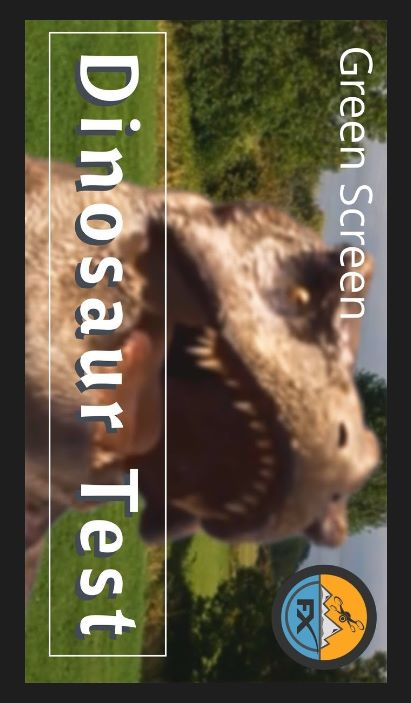
\includegraphics[width=5cm]{Images/Dino-test/dino-testrotate.jpg}\hfill
        \caption{Figuras de Ejemplo}
        \label{fig:ejemplo}
    \end{figure}

    
        
    \newpage
        \begin{algorithm}
            \caption{Rotación Imagen
            }\label{alg:two}
            \KwResult{$imagenRotada$}
            
                
                %print("Perfecto m: i") \;
                
                \eIf{width == 1}{
                    \For{$i\gets0$ \KwTo $ceil(n / 2) + 1$}{
                        invierte pixeles\;
                    }
                }
                { 
                    continue\;
                }
                \eIf{height == 1}{
                    \For{$i\gets0$ \KwTo $ceil(n / 2) + 1$}{
                        invierte pixeles\;
                    }
                
                }{
                    image00 = crop((0, 0, floor(width / 2), floor(height / 2)))\;
                    image01 = crop((floor(width / 2), 0, width, floor(height / 2)))\;
                    image10 = crop((0, floor(height / 2), floor(width / 2), height))\;
                    image11 = crop((floor(width / 2), floor(height / 2), width, height))\;
                    image00 = rotate(image00, clkwise)\;
                    image01 = rotate(image01, clkwise)\;
                    image10 = rotate(image10, clkwise)\;
                    image11 = rotate(image11, clkwise)\;

                    \eIf{clkwise}{
                        image00 = image10\;
                        image10 = image11\;
                        image11 = image01\;
                        image01 = aux\;
                    }{
                        image00 = image01\;
                        image01 = image11\;
                        image11 = image10\;
                        image10 = aux\;

                    }
                
                }
                result.paste(image00, box=(0, 0))\;
                result.paste(image01, box=(image00.size[0], 0))\;
                result.paste(image10, box=(0, image00.size[1]))\;
                result.paste(image11, box=(image00.size[0], image00.size[1]))\;
                return result\;
                
                % \eIf{arreglo[0] == elemento or arreglo[n] == arreglo or arreglo[2*n] == elemento}{
                %     return True\;
                % }
                % \eIf{elemento < arreglo[n]}{
                %     arreglo = arreglo[0:n]\;
                % }
                % \eIf{elemento < arreglo[n*2]}{
                %     arreglo = arreglo[n:n*2]\;
                % }
                % {
                %     arreglo = arreglo[n*2:n*3]\;
                % }
            
        \end{algorithm}
        
        
        
        